\section{Physical layer in \mbox{Mote Runner}}
\begin{frame}[fragile]
  \frametitle{Radio interface - 1}
  \begin{itemize}
    \item MR v.13 offers a Radio interface IEEE 802.15.4 compliant
    \begin{itemize}
    	\item It is a generic class in the IBM saguaro system that permits to use the radio device
    	\item It offers an API with the following functionality:
    	\begin{itemize}
			\item open: opens the radio, once opened no other assembly can use it
			\item close: releases the radio so that others can use it
			\item setter and getters for channel and network parameters (addresses, panid...)
			\item startReceive: listens the channel (in one of the many receiption mode)
			\item transmit: begin to transmit a pdu
    	\end{itemize}
    \end{itemize}
  \end{itemize}
\end{frame}

\begin{frame}[fragile]
	\frametitle{Radio interface - 2}
	\begin{itemize}
		\item In addition Radio:
		\begin{itemize}
			\item Handles transmission and receiption notifing to higher level by delegation
			\item Manages acks notifing failure or success states in callbacks
			\item Permits to set parameters as PAN identifier, short address, radio channel
			\item Permits to register functions that will handle the radio events (Tx and Rx)
		\end{itemize}
	\end{itemize}
\end{frame}


\begin{frame}[fragile]
  \frametitle{Transmission \& Reception - 1}
  \begin{itemize}
    \item These operations require much attention:
    \begin{itemize}
    	\item Radio permits to transmit every type of pdu, but it's possible to receive only packets with 802.15.4 well formed headers
    	\item It's also possible to receive in promiscuous mode to sniff for every packet, but this exposes to interferences
    \end{itemize}
    \item Each mote holds 3 addresses:
    \begin{itemize}
    	\item a 16-bit PAN identifier
    	\item a 64-bit extended address that uniquely identifies a mote
    	\item a 16-bit short address that's application and protocol specific
    \end{itemize}
  \end{itemize}
\end{frame}

\begin{frame}[fragile]
  \frametitle{Transmission \& Reception - 2}
  \begin{figure}
  	\centering
  	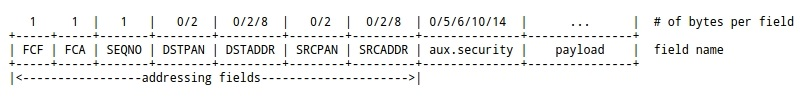
\includegraphics[width=\textwidth]{img/header.jpg}
  	\caption{PDU header format}
  \end{figure}
  \begin{columns}
  	\begin{column}{.52\textwidth}
	    \begin{figure}
	    	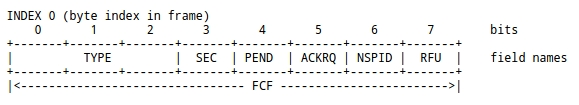
\includegraphics[width=\textwidth]{img/fcf.jpg}
  		\caption{Frame Control Flags}
	    \end{figure}
  	\end{column}
  	\hfill
	\begin{column}{.45\textwidth}
	    \begin{figure}
	    	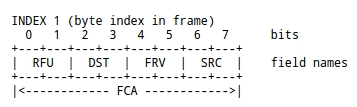
\includegraphics[width=\textwidth]{img/fca.jpg}
  		\caption{Frame Control Address Flags}
	    \end{figure}
  	\end{column}
  \end{columns}
\end{frame}
% 
% \begin{frame}[fragile]
%   \frametitle{Tx/Rx - Filtering}
%   \begin{itemize}
%     \item Possible packets are specified in FCF-Type field and are: BEACON, DATA, ACK and CMD.
%     \item BEACONs are accepted only if the header field SRCPAN matches the mote's PANID or it's BROADCAST
%     \item If FCA Flags specify an address then 
%   \end{itemize}
% \end{frame}

\begin{frame}[fragile]
  \frametitle{Tx/Rx Real and Real Time Constraints}
  \begin{itemize}
    \item It's possible to operate in many different ways with regards to real time constraints:
    \begin{itemize}
    	\item It's possible to receive/transmit ASAP (As Soon As Possible) or EXACTLY at the specified time or ...
    	\item Rx/Tx require a start operation time and an end one
    	\item MR manages autonomously all warm up and ramp up to make the device ready at the specified time
    	\item The device turn off at the end and an event is raised to be managed with delegation
    	\item If the device cannot be ready at the specified time or an error occurs which reports this status
    \end{itemize}

  \end{itemize}
\end{frame}